\documentclass[12pt]{article}

\usepackage{graphicx}
\usepackage{caption}
\usepackage[font=normalsize]{subcaption}
\usepackage{float}
\usepackage{setspace}
\usepackage{booktabs}
\usepackage{wrapfig}

% spacing surround wrapfigs
\setlength{\columnsep}{12pt}

% bold the 'Figure~#' in the caption and separate it with a period
% Captions will be left justified
\usepackage[labelsep=period,font=small,labelfont=bf]{caption}

%%% STYLING %%%%%%%%%%%%%%%%%%%%%%%
\usepackage[compact]{titlesec}
\titleformat{\subsection}{\normalfont\fontsize{13}{15}\bfseries}{\thesubsubsection}{1em}{}
\titleformat{\subsubsection}{\normalfont\fontsize{12}{15}\bfseries}{\thesubsubsection}{1em}{}
\titleformat{\paragraph}[runin]{\normalfont\bfseries}{\theparagraph}{3pt}{}[ $\;\cdotp\;$]
\titlespacing{\paragraph}{0pt}{*1}{*0.5}
\usepackage{parskip}
\setlength{\parskip}{0.15cm}
%%%%%%%%%%%%%%%%%%%%%%%%%%%%%%%%%%%

\begin{document}

\section{Identifying optimal LBI parameters}

To determine the optimal tau and window parameters for the LBI fitness predictor, I ran a parameter sweep for all possible combinations of tau and window values across a range of both parameters.
I tested tau values of 0.03125, 0.0625, 0.125, 0.25, 0.5, 0.75, 1.0 and window values of 0.1, 0.25, 0.75.
I evaluated the accuracy of each combination of tau and window values by running the fitness model with the LBI predictor on a tree with 92 viruses per month across Oct 2006--Apr 2018 and measuring the frequency fold change correlation and Matthew's correlation coefficient (MCC) for growth or decline of clade frequencies.
The first of these two metrics measures how well the model predicts the specific change in frequency for each clade.
The second metric measures how well the model predicts that a clade will grow or decline in frequency.

\begin{figure}[h]
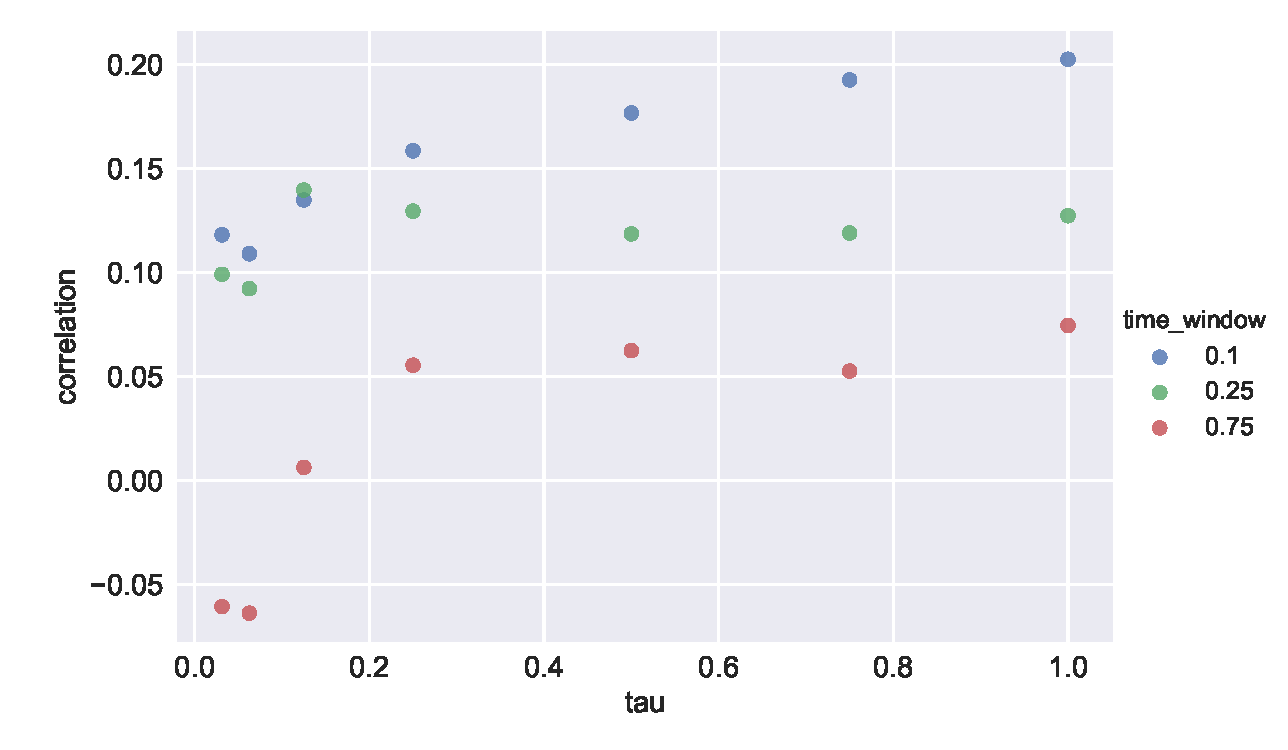
\includegraphics[width=5in]{frequency_correlation_by_lbi_parameters.pdf}
\caption{\label{fig:frequency-correlation-by-lbi-parameters}Correlation of predicted and observed frequency fold change by LBI parameters}
\end{figure}

\begin{figure}[h]
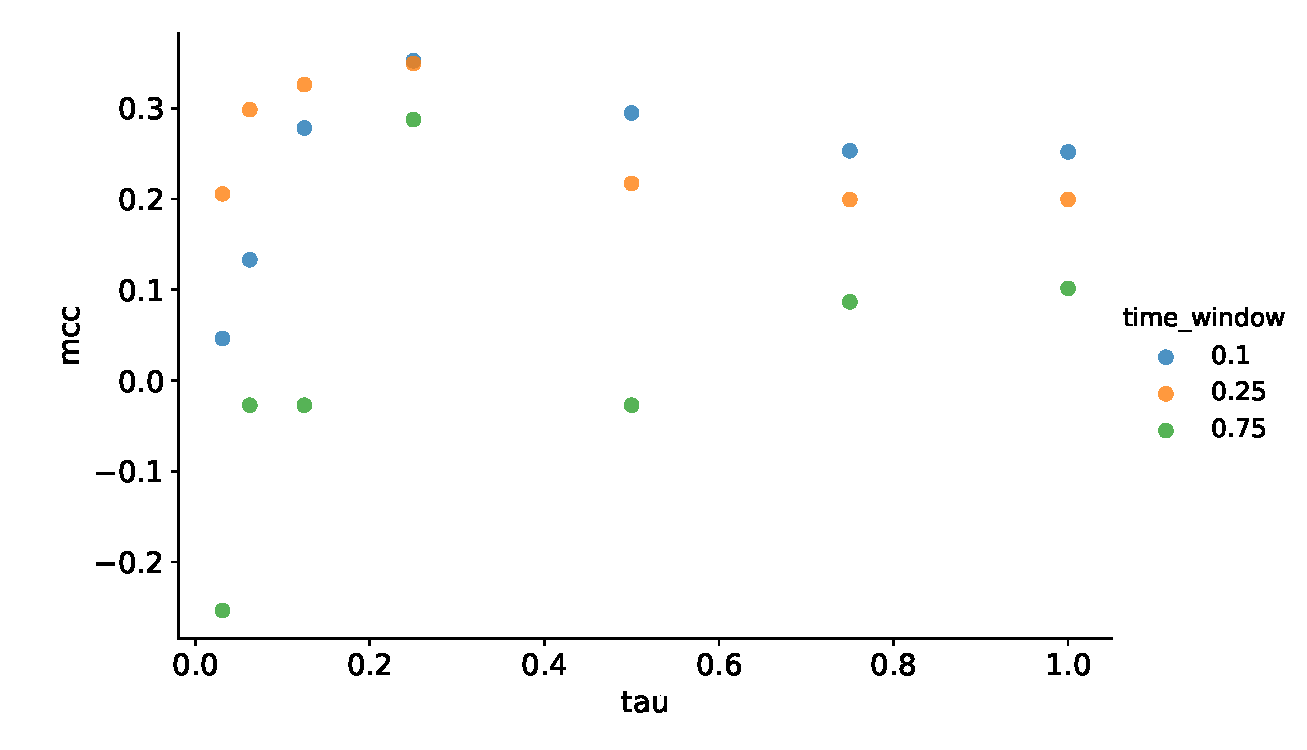
\includegraphics[width=5in]{mcc_by_lbi_parameters.pdf}
\caption{\label{fig:mcc-by-lbi-parameters}Matthew's correlation coefficient (MCC) by LBI parameters}
\end{figure}

The model performed best by correlation (0.20) with tau of 1.0 and window of 0.1 (Fig.~\ref{fig:frequency-correlation-by-lbi-parameters}).
The model performed best by MCC (0.35) with tau of 0.25 and a window of 0.1 or 0.25 (Fig.~\ref{fig:mcc-by-lbi-parameters}).
Importantly, the current LBI parameters for 12 year trees (tau of 0.75 and window of 0.75) performed poorly by both correlation (0.06) and MCC (0.02).
The longest time window (0.75) produced the worst MCCs for all values of tau.
For tau greater or equal to 0.125, the window sizes of 0.1 and 0.25 were almost equally accurate.
Since LBI is not expected to perform well in predicting specific clade frequencies but rather in predicting clade growth or decline, I opted to select the LBI parameters that maximized the MCC (tau of 0.25 and window of 0.1).

To understand how these new LBI parameters change the annotations of recent clades, I ran LBI with both the standard settings (tau of 0.75, window of 0.75) and the new optimal settings on a tree with 92 viruses per month from 2016--2018 and visualized the results in auspice.
The standard LBI parameters clearly highlight the rapid emergence of the A2/re clade over the last year (Fig.~\ref{auspice-lbi-with-standard-parameters}).
In contrast, the optimal LBI parameters for the fitness model identify recent rapid branching in one small subclade of A1b/135K (Fig.~\ref{auspice-lbi-with-optimal-parameters}).

\begin{figure}[h]
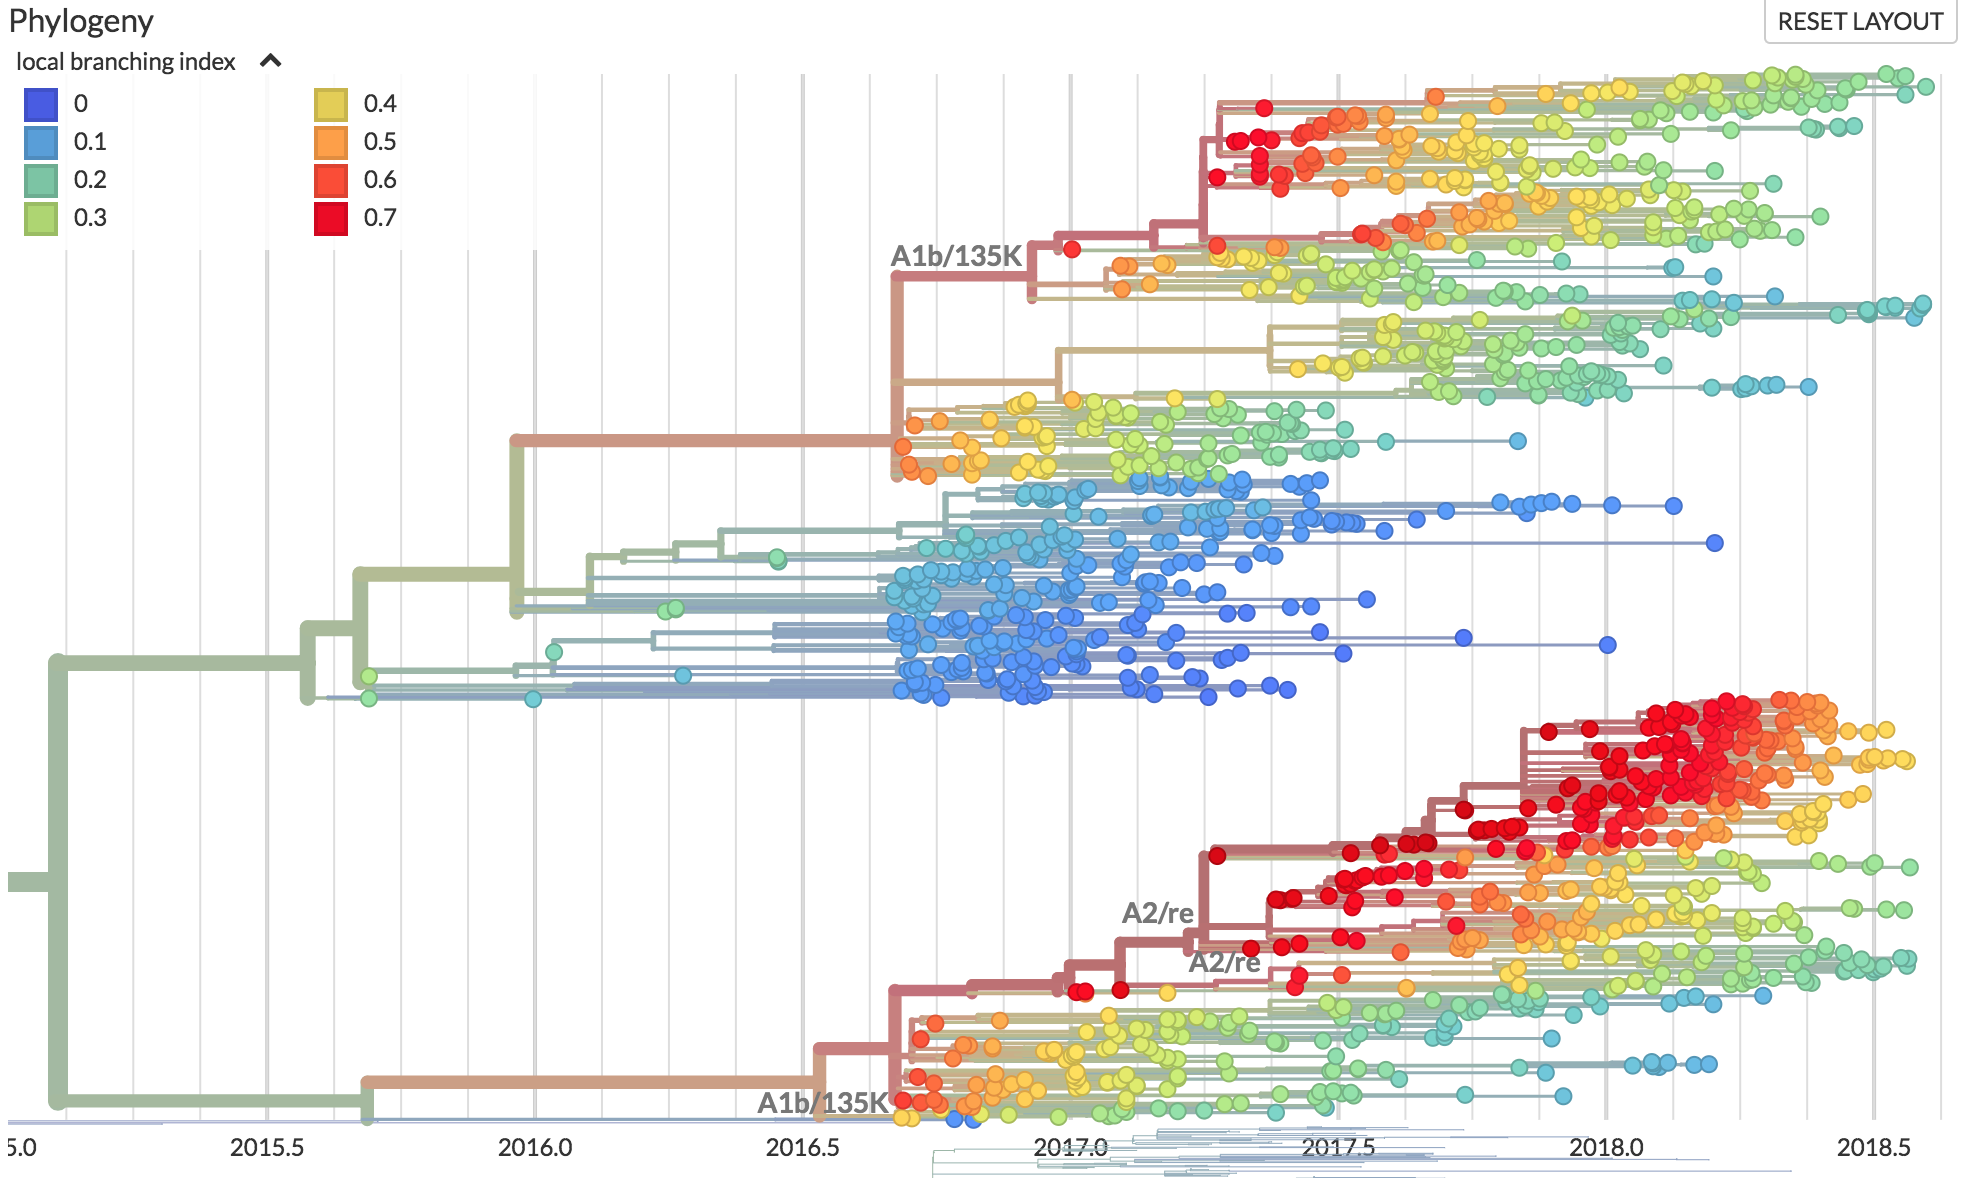
\includegraphics[width=5in]{auspice-lbi-tau-0-75-window-0-75.png}
\caption{\label{auspice-lbi-with-standard-parameters}Auspice view of recent clades with standard LBI parameters (tau = 0.75, window = 0.75)}
\end{figure}

\begin{figure}[h]
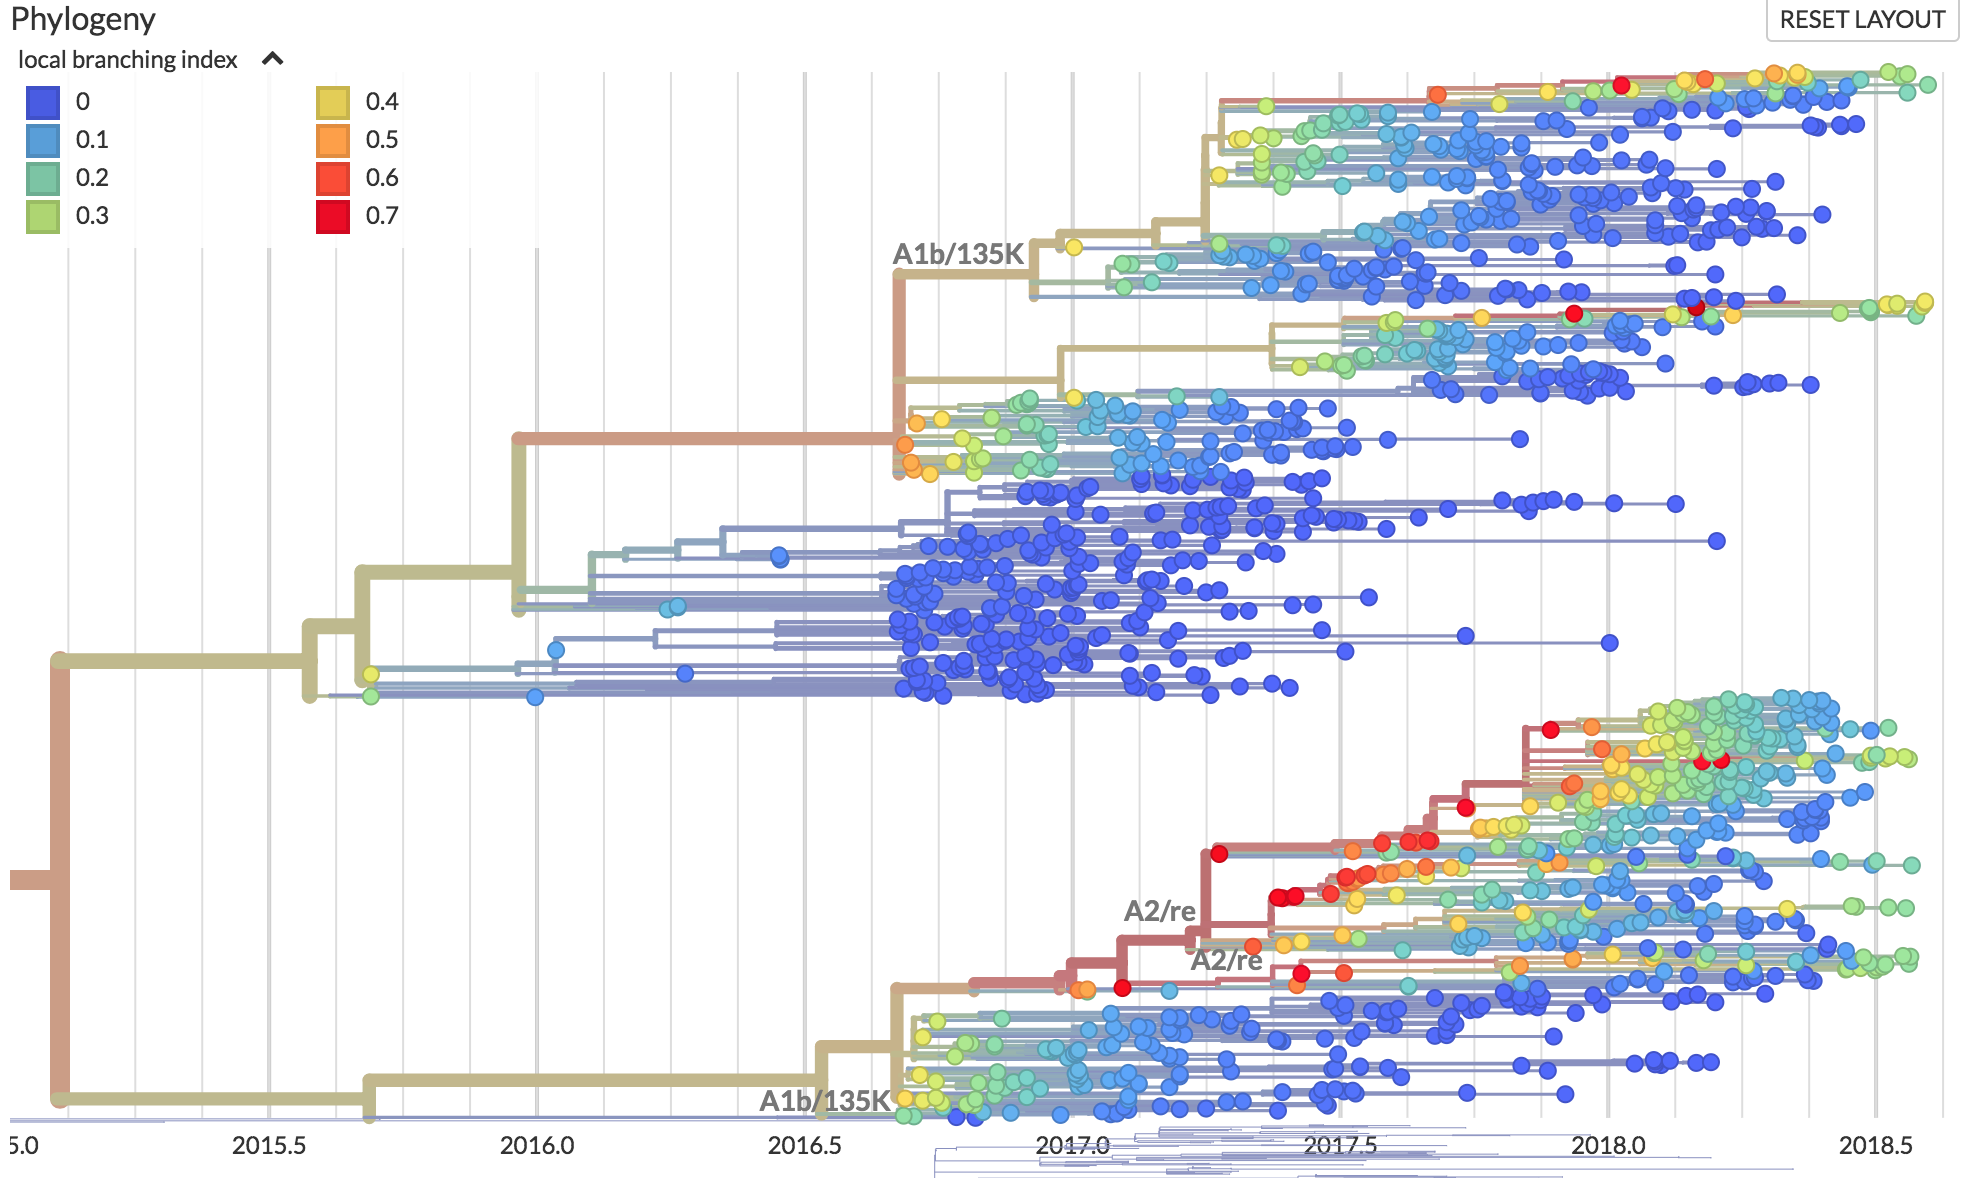
\includegraphics[width=5in]{auspice-lbi-tau-0-25-window-0-1.png}
\caption{\label{auspice-lbi-with-optimal-parameters}Auspice view of recent clades with optimal LBI parameters (tau = 0.25, window = 0.1)}
\end{figure}

After standardization of LBI values across all tips in the most recent timepoint of the fitness model, the A2/re clade has much lower LBI values than the A1b/135K clade (Fig.~\ref{fitness-tree-with-lbi-predictor}).

\begin{figure}[h]
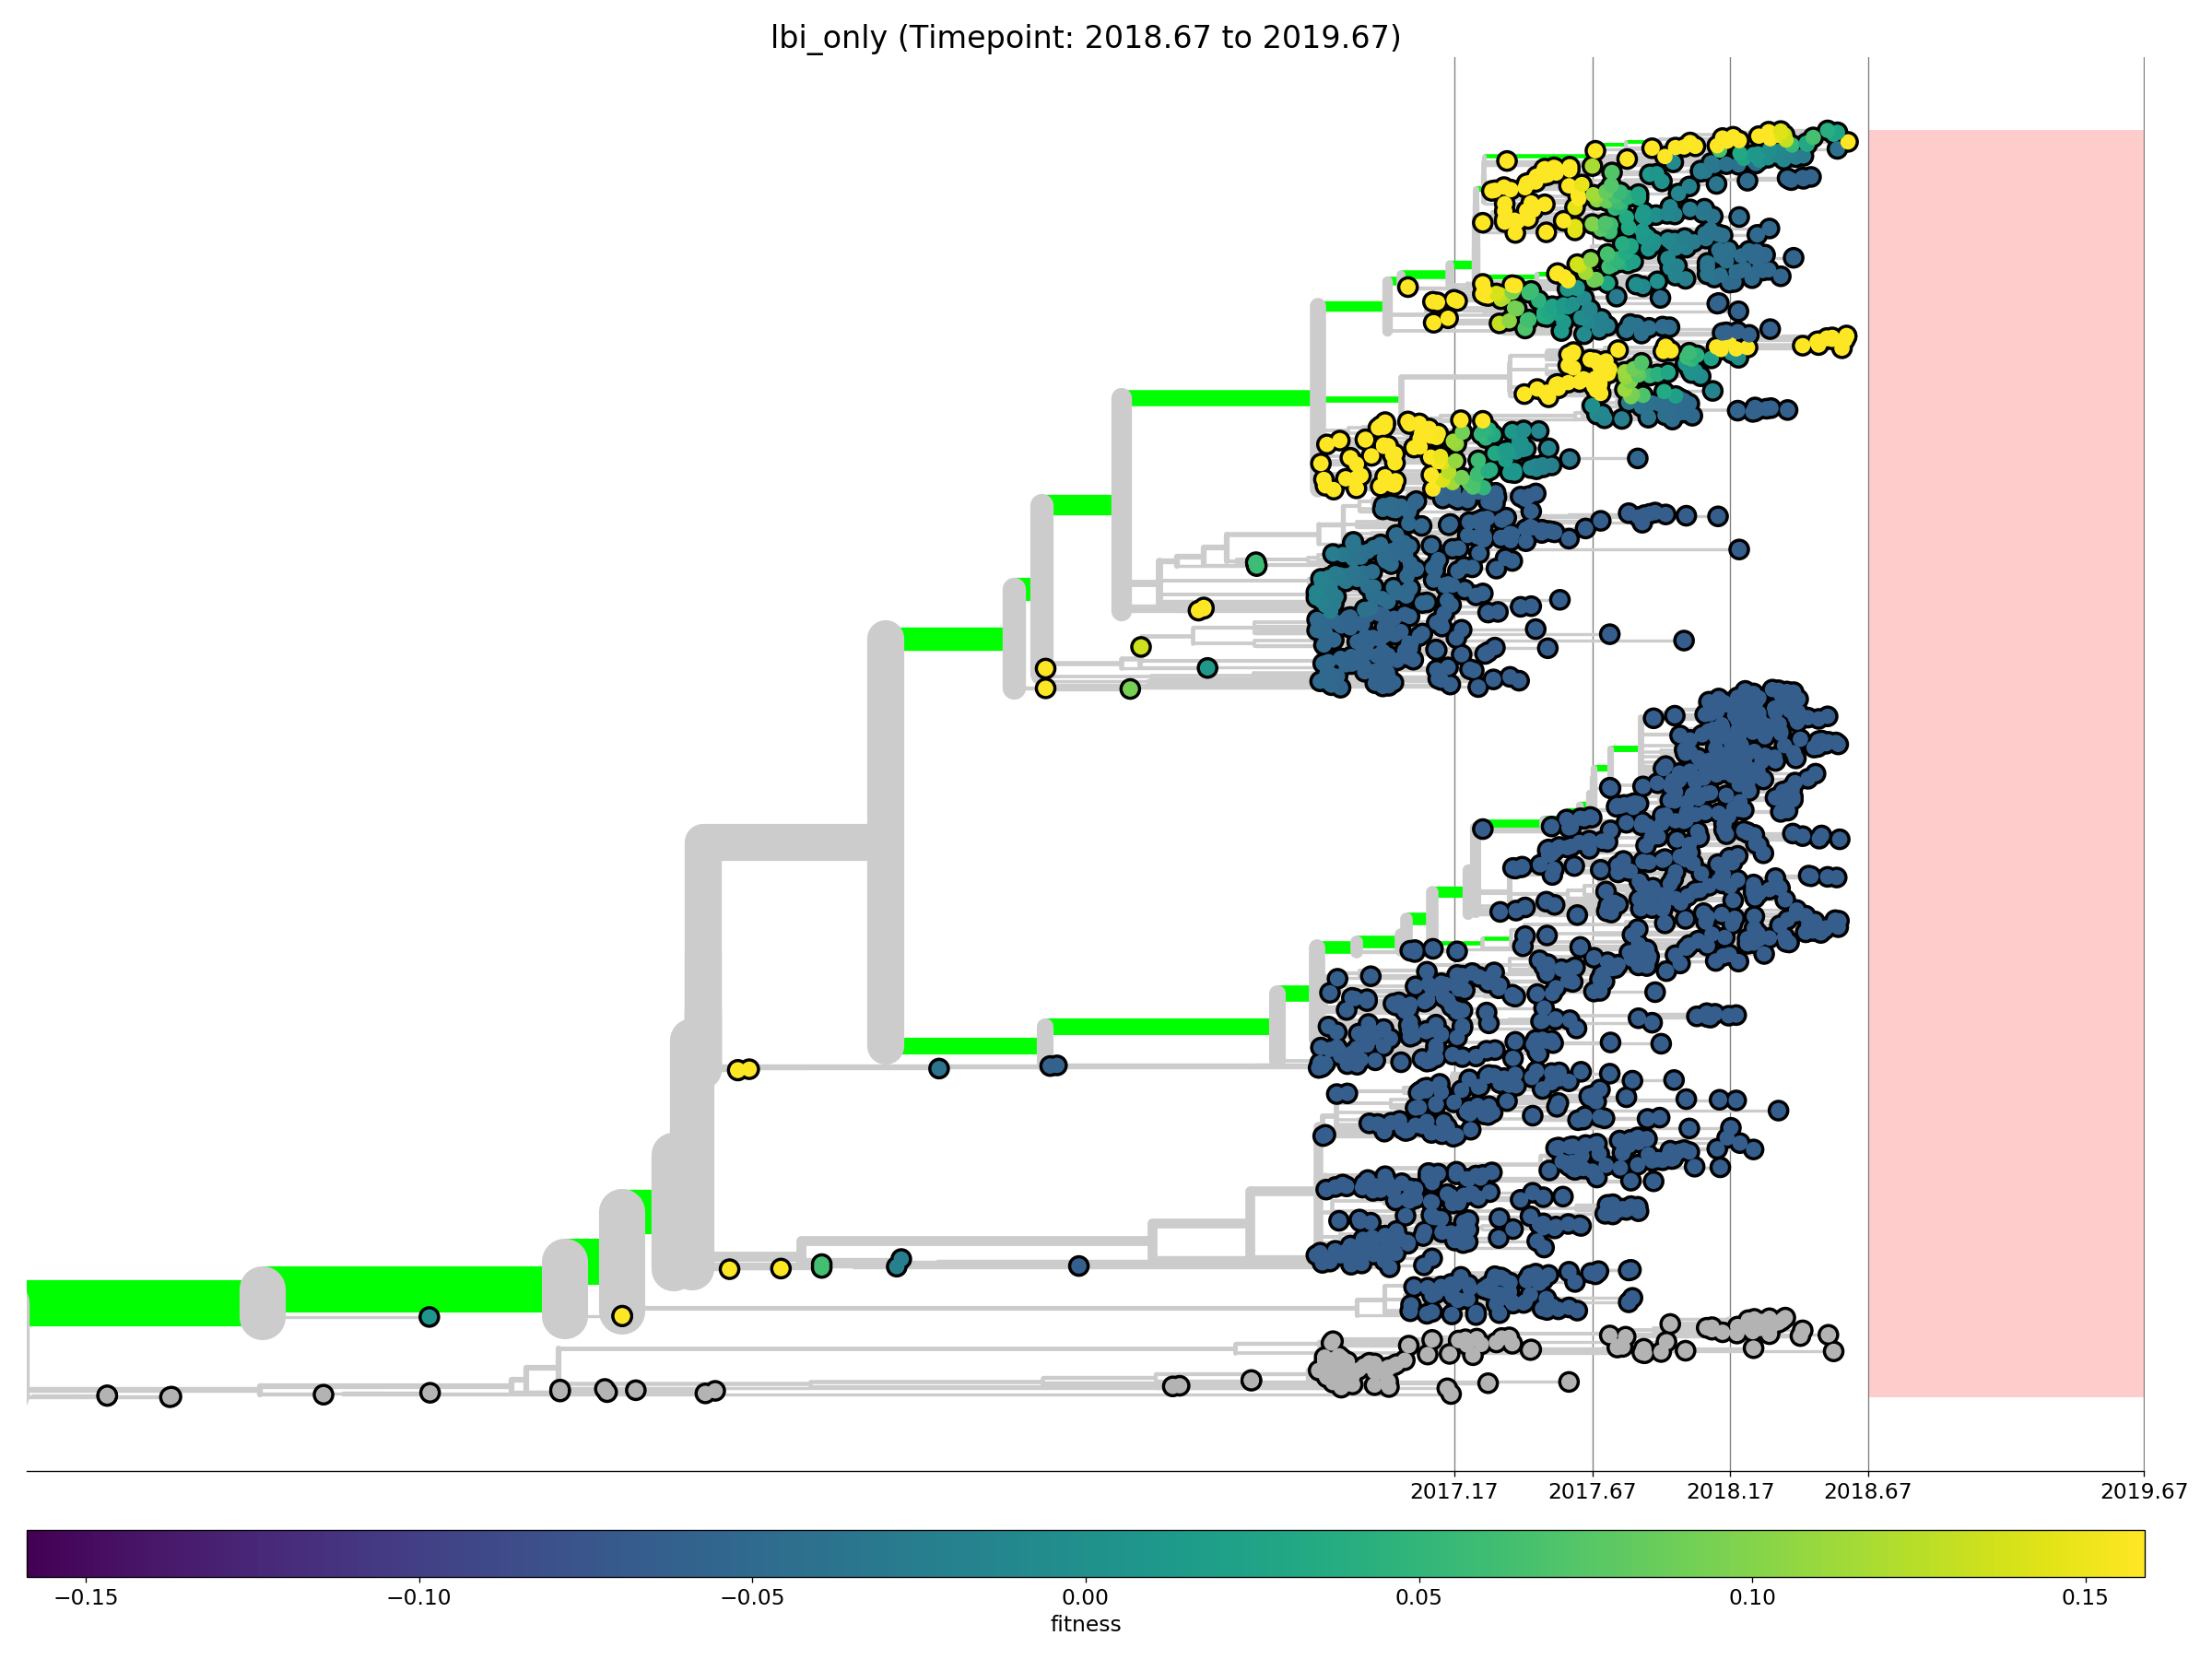
\includegraphics[width=5in]{h3n2-ha-fitness-phylogeny-lbi_2018-67.png}
\caption{\label{fitness-tree-with-lbi-predictor}BALTIC view of recent clades with LBI calculated from new optimal parameters and standardized across all tips in the current timepoint.}
\end{figure}

\section{Model performance}

I ran the forecasting builds with all predictors and the new optimal LBI parameters.
In addition to the standard ``all'' predictor that includes all individual predictors, I added a predictor based on the titer substitution model and LBI and another based on titers, LBI, and non-epitope mutations.
The models with the best correlation and MCC values were consistently those with titer substitution predictors (Fig.~\ref{fig:model-frequency-correlations} and \ref{fig:model-mcc}).

\begin{figure}
\includegraphics[width=5in]{../../figures/frequency_correlation.pdf}
\caption{\label{fig:model-frequency-correlations}Pearson's correlation between observed and predicted frequency fold change by fitness predictors.}
\end{figure}

\begin{figure}
\includegraphics[width=5in]{../../figures/mcc.pdf}
\caption{\label{fig:model-mcc}Matthew's correlation coefficient (MCC) for clade growth or decline predictions by fitness predictors.}
\end{figure}

By itself, the LBI predictor has a small, positive $\beta$ value of 0.15 (Fig.~\ref{fig:model-parameters}) and a relatively low correlation of 0.16 (Fig.~\ref{fig:model-frequency-correlations}).
However, LBI also has the second highest MCC (0.35) after the titer substitution model indicating that it generally does a better job of predicting clade growth or decline (Fig.~\ref{fig:model-mcc}).
In combination with other predictors, LBI has a larger, negative $\beta$ with the largest value of -0.34 in the combined titers and LBI model.
Despite this negative $\beta$ parameter for LBI, its inclusion with the titer substitution model produces a better MCC than either individual predictor.

\begin{figure}
\includegraphics[width=5in]{../../figures/model_parameters.pdf}
\caption{\label{fig:model-parameters}Model parameters for all combinations of fitness predictors.}
\end{figure}

To understand why the LBI predictor had such a low overall correlation between predicted and observed frequency change, I inspected these predicted and observed values by groups of clades at different initial frequencies.
For each group of clades, I recalculated the Pearson's correlation and Matthew's correlation coefficient.
LBI performs best with medium- to large-sized clades with an initial frequency greater than 50\% (Fig.~\ref{fig:model-fold-change-lbi}).
For clades with an initial frequency less than 50\%, LBI is often overly optimistic about future clade growth.

\begin{figure}
\includegraphics[width=5in]{../../model_fold_change/2006-2018/92/lbi/0.pdf}
\caption{\label{fig:model-fold-change-lbi}Observed and predicted frequency fold change for LBI predictor.}
\end{figure}

In contrast with the LBI predictor, the titer substitution model predictor is less likely to predict that clades will grow when they do not (Fig.~\ref{fig:model-fold-change-cTiterSub}).
Combining the LBI and titer substitution predictors together decreases the model's accuracy in predicting clade growth or decline for clades at greater than 50\% initial frequency, but it increases the model's accuracy with clades at less than 50\% frequency (Fig.~\ref{fig:model-fold-change-cTiterSub-lbi}).

\begin{figure}
\includegraphics[width=5in]{../../model_fold_change/2006-2018/92/cTiterSub/0.pdf}
\caption{\label{fig:model-fold-change-cTiterSub}Observed and predicted frequency fold change for titer substitution predictor.}
\end{figure}

\begin{figure}
\includegraphics[width=5in]{../../model_fold_change/2006-2018/92/cTiterSub-lbi/0.pdf}
\caption{\label{fig:model-fold-change-cTiterSub-lbi}Observed and predicted frequency fold change for titer substitution and LBI predictors.}
\end{figure}

\begin{figure}
\includegraphics[width=5in]{../../model_fold_change/2006-2018/92/ne-cTiterSub-lbi/0.pdf}
\caption{\label{fig:model-fold-change-ne-cTiterSub-lbi}Observed and predicted frequency fold change for non-epitope mutations, titer substitution, and LBI predictors.}
\end{figure}

\section{Forecasts with LBI predictors}

Using the optimal LBI parameters for the fitness model, the clade A1b/135K has higher standardized LBI values than A2/re (Fig.~\ref{fig:relative-clade-fitnesses}).
A1b/135K has higher standard values for all three metrics from the best fit model (non-epitopes, titer substitutions, and LBI).
As a result, this clade also has a higher overall fitness and is projected to increase in frequency by the best fit model (Fig.~\ref{fig:projected-global-clade-frequencies}).
The only models that do not project a decline in A2/re are the LBI and sequence-only models which project a slight decline or no change over the next year.

\begin{figure}
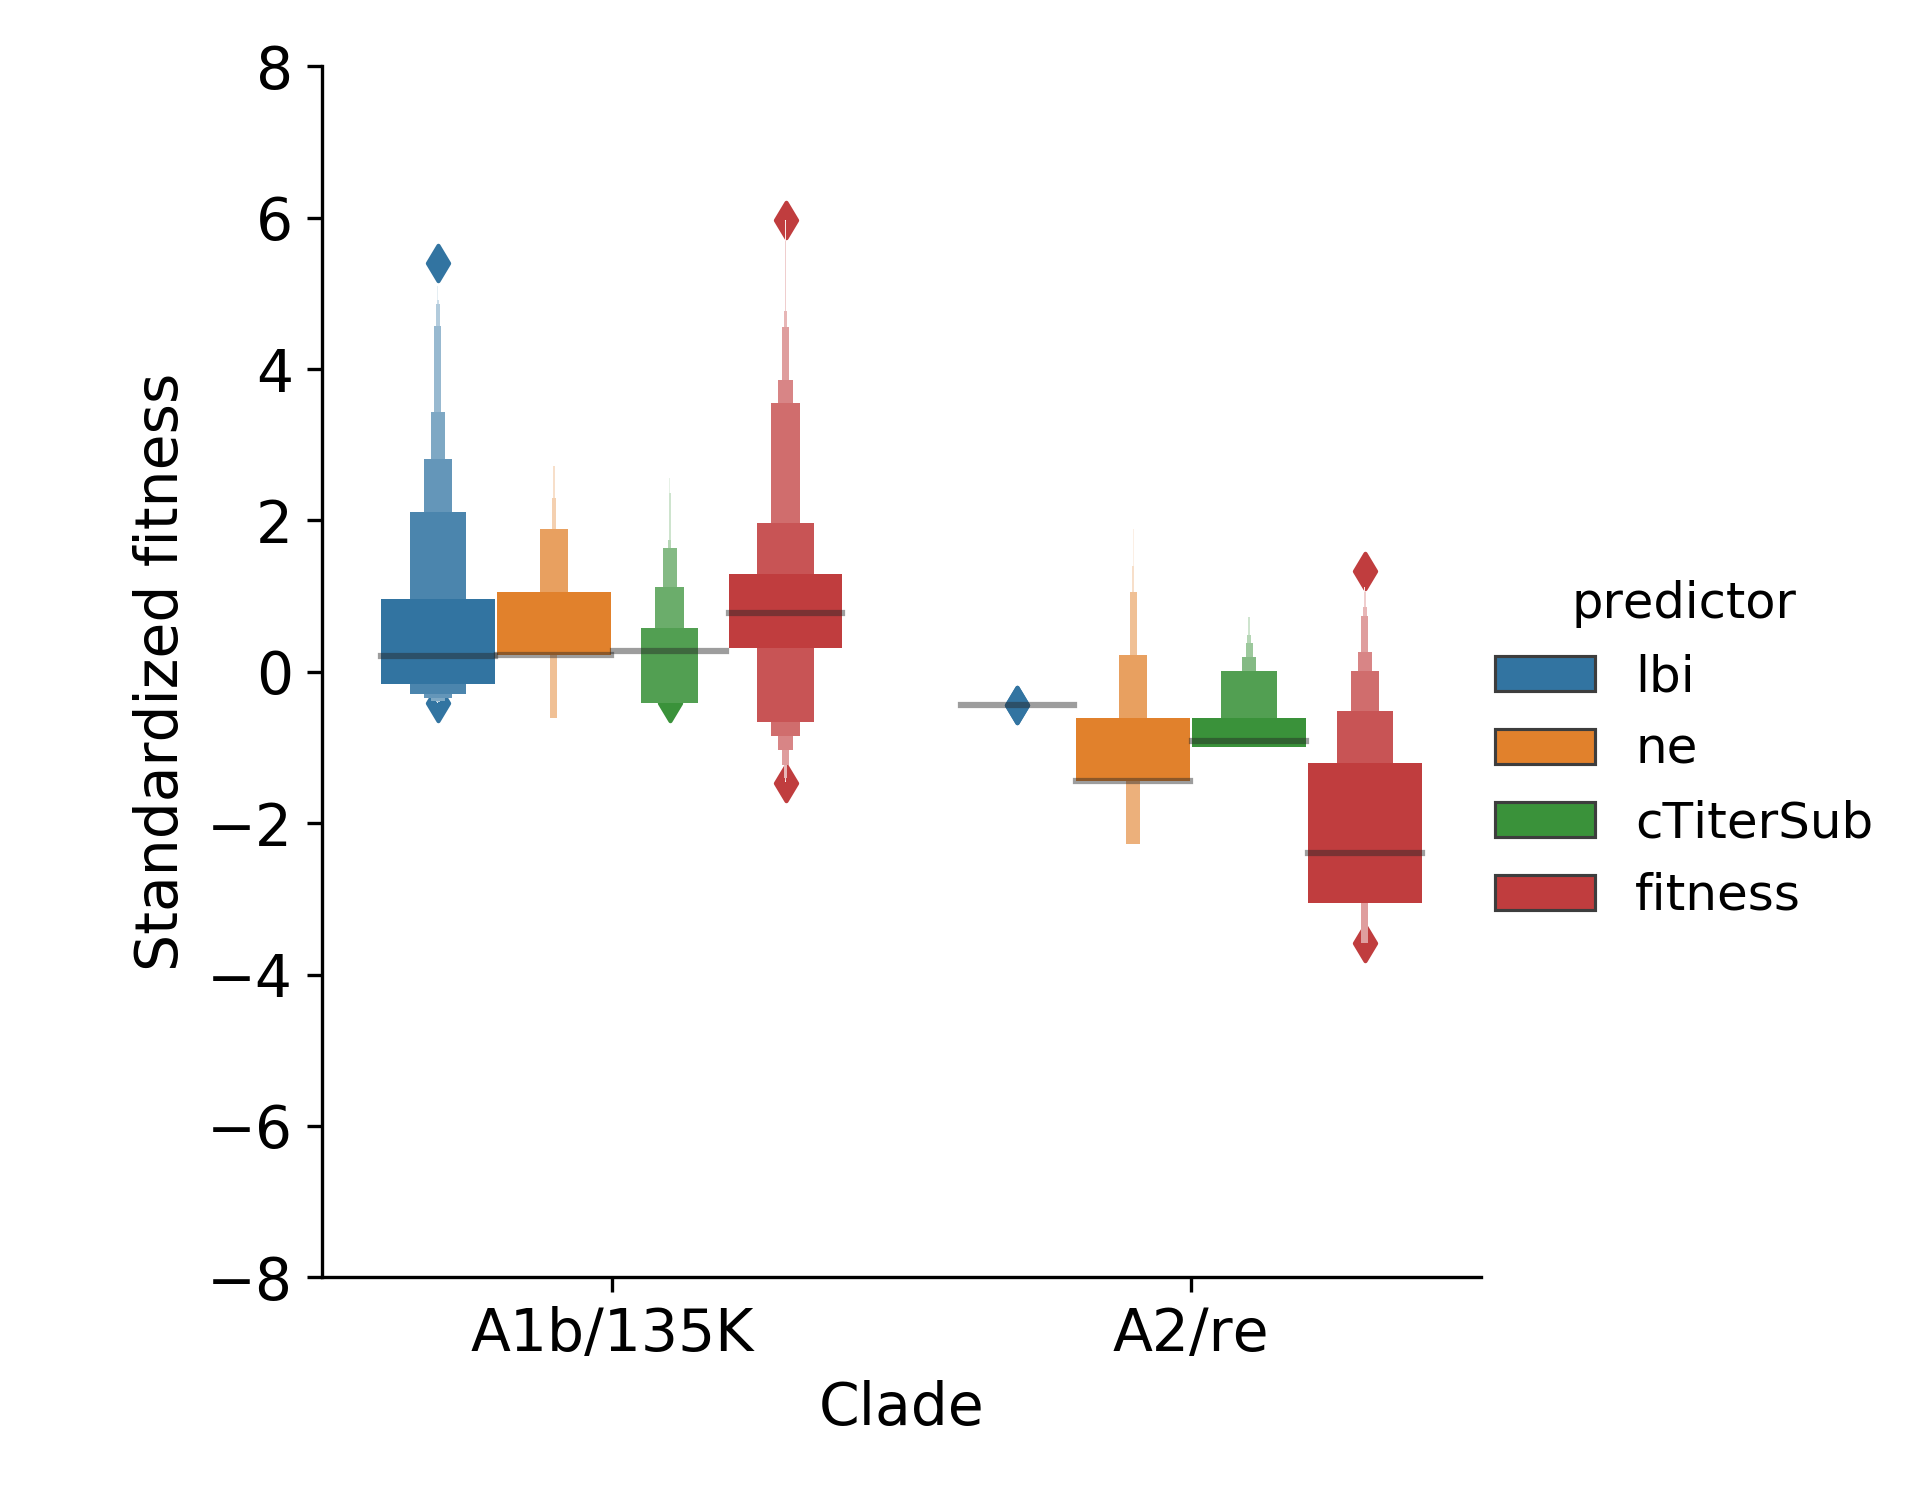
\includegraphics[width=5in]{h3n2-ha-relative-clade-fitnesses.png}
\caption{\label{fig:relative-clade-fitnesses}Standardized fitness metrics by clade and overall fitness based on model parameters for the non-epitope, titer substitution, and LBI model.}
\end{figure}

\begin{figure}
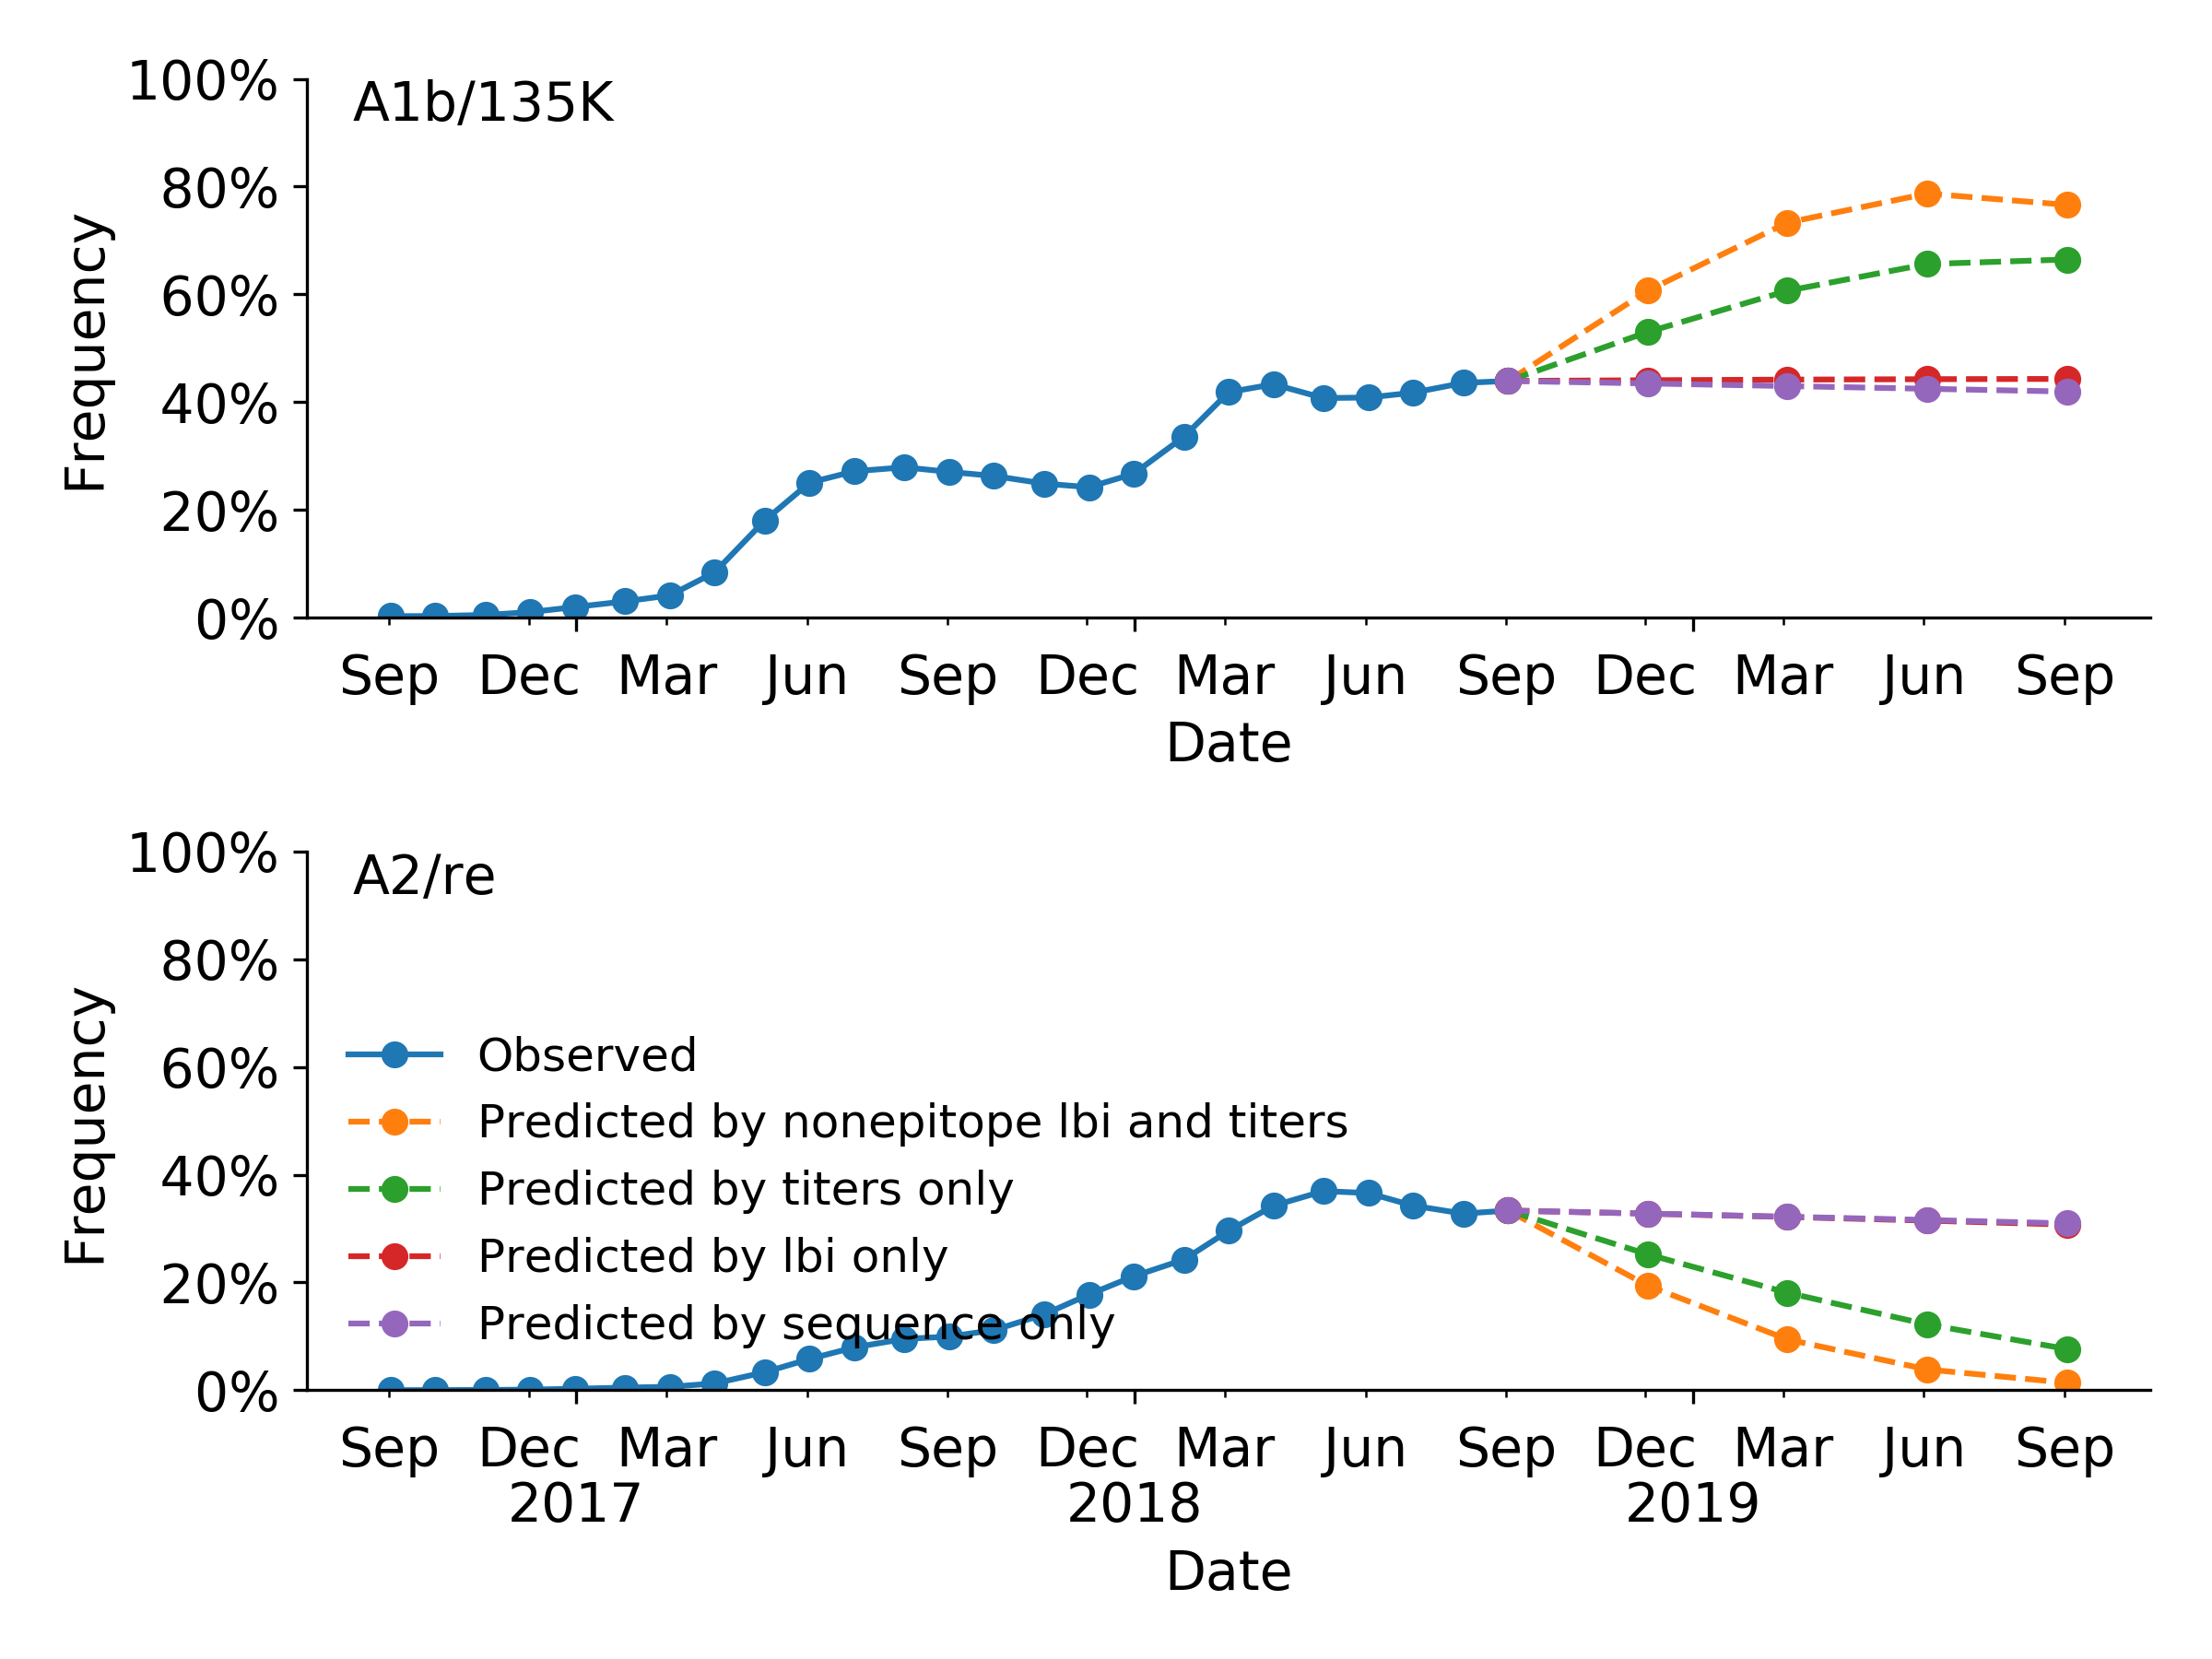
\includegraphics[width=5in]{h3n2-ha-projected-global-frequencies-by-clade.png}
\caption{\label{fig:projected-global-clade-frequencies}Projected global clade frequencies.}
\end{figure}

\end{document}
